\begin{frame}{Our challenge and philosophy}
\key{A reconstruction loss rewards every pixel}\par
Drawing a cross beside a 7 lowers pixel error. The cross carries no intended information about which digit was written.
\par\bigskip
\key{A digit's cluster should survive a change of decoration}\par
Give the decoder a stronger incentive to reproduce the central handwriting, or show it transformed versions of each image. Measure what happens when only the cross moves.
\notefoot{Each symbol adds nine pixels to verified blank space. All handwriting stays intact, including faint edges.}
\end{frame}

\begin{frame}{What changes during training and testing?}
\centering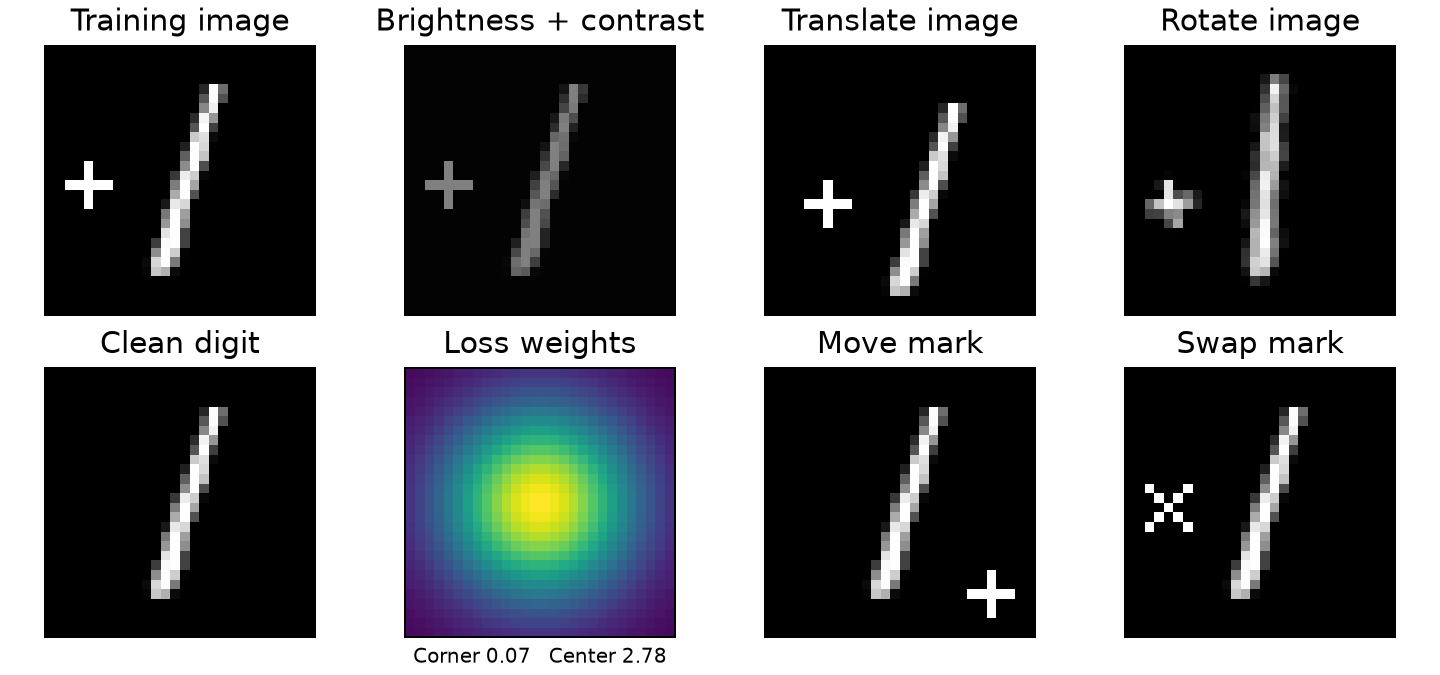
\includegraphics[width=.89\linewidth,height=.73\textheight,keepaspectratio]{../figures/photometric.png}
\notefoot{Training transforms the entire marked image. The two background tests change the decoration while holding the handwriting fixed.}
\end{frame}

\begin{frame}{Separating digit accuracy from background sensitivity}
\begin{columns}[T,onlytextwidth]
\column{.47\textwidth}\key{Train on marked digits}\par\medskip
Test brightness/contrast jitter, whole-image translation and small rotation. For each, turn the Gaussian loss weights on and off. Ordinary IDEC and Gaussian alone are shared controls.
\column{.47\textwidth}\key{Train on clean digits}\par\medskip
Repeat ordinary IDEC and each augmentation with no symbol present. A clean-test accuracy gain shows that the method can improve clustering even in the absence of the mark.
\end{columns}
\par\bigskip
\notefoot{12 arms, five matched seeds, 12,000 training and 10,000 test digits. Only pretraining changes. Digit labels are used for evaluation after fitting.}
\end{frame}

\begin{frame}{Can we read the mark from the digit representation?}
\key{Assignments}\par
Move the symbol, or swap its shape at the same site. Count how often the frozen IDEC model changes its cluster.
\par\bigskip
\key{Representation}\par
Show both a plus and a cross for every training digit at the same location. Fit a linear probe on the final embeddings. Test whether it can identify the symbol on unseen digits. Chance is 50\%.
\notefoot{The probe uses synthetic shape labels only after IDEC training. A model can retain shape information even when its cluster assignment stays the same.}
\end{frame}

\begin{frame}{Which standalone intervention stabilizes the clusters?}
\centering\small\setlength{\tabcolsep}{3pt}\begin{tabular}{lrrrrr}
\toprule
Pretraining & Marked ACC & Clean ACC & Move flips & Shape flips & Shape probe\\
\midrule
Ordinary IDEC & 67.51 & 70.22 & 6.23 & 5.36 & 50.20\\
Jitter only & 68.64 & 71.14 & 6.06 & 4.98 & 50.26\\
Translation & 80.63 & 81.61 & 3.41 & 2.73 & 50.21\\
Rotation & 74.01 & 76.08 & 5.05 & 4.00 & 50.15\\
Gaussian only & 71.42 & 73.47 & 5.19 & 4.53 & 50.13\\
\bottomrule
\end{tabular}

\par\bigskip\normalsizeTranslation surpassed Gaussian weighting in every seed on marked accuracy and on both background-switch tests. Shape probe accuracy remained near chance.

\notefoot{Five-seed means, in percent. Each row uses one marked training image per digit. The standalone Gaussian weights errors around the image center during reconstruction.}
\end{frame}

\begin{frame}{Does augmentation help when no mark is present?}
\centering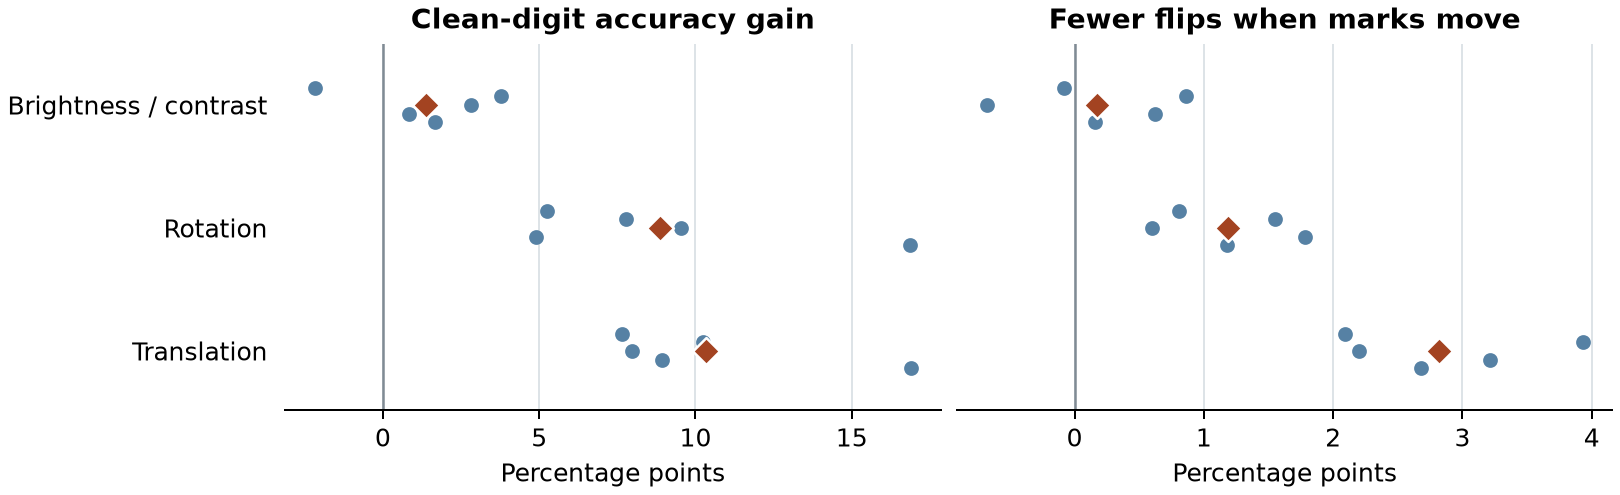
\includegraphics[width=.98\linewidth,height=.64\textheight,keepaspectratio]{../figures/augmentation_effects.png}
\notefoot{Each blue point is one matched seed. The diamond is its five-seed mean. Positive values indicate improvement in each panel. Clean-only accuracy uses separate models trained and tested without geometric marks.}
\end{frame}

\begin{frame}{Choosing a solution for digit clustering}
\key{Use small random translations during pretraining}\par
Against Gaussian weighting alone, translation gained 9.21 percentage points in marked-digit accuracy and reduced movement flips by 1.78 points. All five seeds agreed on both comparisons. Adding Gaussian weighting to translation gave 79.93\% accuracy, compared with 80.63\% for translation alone.
\par\bigskip
\key{Two effects coexist}\par
When no mark appeared in training or testing, translation still raised digit accuracy from 73.53\% to 83.87\%. With marks present in training it also stabilized assignments when only the background changed. The shape probe was near chance under every standalone method.
\notefoot{The results support improved digit clustering and reduced sensitivity to these marks. They leave the amount of background information retained in the embedding unresolved.}

\end{frame}
